%%  This is the driver file for working group reports contributed 
%%   to the Snowmass 2013 proceedings

%%  This file includes brings in all the necessary files to provide the
%%  format of the Proceedings
%%
%%  D. Hitlin   9/23/03   derived from the BABAR Physics Book format

%%  Please do not change anything in this file, except to include the
%%  name of your file on the next to last line of this file

%%  To use LATEX with this format, you must have the follwing files 
%%  in the same directory as your text source and figure files
%%  tcibook.cls
%%  fancyhea.sty
%%  work.sty
%%  epsfig.sty
%%  workshopsym.tex       This file provides macros for many common symbols
%%                         Using these macros will provide uniformity of notation
%%                         for the basic particle symbols, units, etc.
%%
%%  These provide the page size, type style, headings, etc.


\documentclass{tcibook}
\usepackage{fancyhea}
\usepackage{work}
\usepackage{bm}       %    enables bold math symbols  e.g.  \bm{\gamma}
\usepackage{graphicx}
\usepackage{hyperref} 
%Added for ChargedLeptons
\usepackage{xspace}
\usepackage{placeins}
\usepackage{multirow}
%\usepackage{draftwatermark}
%\SetWatermarkScale{5}
%\SetWatermarkLightness{0.9}

% hypertext links %%ARXIV

\input workshopsymbols.tex      %   standard macros for common HEP terms

\setlength{\headheight}{14pt}

% subsubsections are numbered as well as chapters, sections and subsections.
\setcounter{secnumdepth}{4}

\begin{document}

\def\bibname{References}
\bibliographystyle{plain}

\raggedbottom

\pagenumbering{roman}

\parindent=0pt
\parskip=8pt
\setlength{\evensidemargin}{0pt}
\setlength{\oddsidemargin}{0pt}
\setlength{\marginparsep}{0.0in}
\setlength{\marginparwidth}{0.0in}
\marginparpush=0pt

% The content begins here

\pagenumbering{arabic}

\renewcommand{\chapname}{chap:intro_}
\renewcommand{\chapterdir}{.}
\renewcommand{\arraystretch}{1.25}
\addtolength{\arraycolsep}{-3pt}




\chapter{Executive Summary\break Charged Leptons}
\bigskip\bigskip
The enormous physics potential of the charged
lepton experimental program was very much in evidence at the Workshop. There are discovery opportunities in experiments that will be conducted over the coming decade using existing facilities and in more sensitive experiments possible with future facilities such as Project X.
Exquisitly sensitive searches for rare decays of muons and tau leptons, together with precision measurements of their properties will either elucidate the scale and dynamics of flavor generation, or
limit the scale of flavor generation to well above $10^4$ TeV.  

The crown jewel of the program is the discovery potential of muon and tau decay experiments searching for charged lepton flavor violation (CLFV) with several orders-of-magnitude improvement in sensitivity in
multiple processes.  There is an
international program of CLFV searches, with experiments recently completed, currently running, and
soon to be constructed in the United States, Japan, and Europe.  These include the completion of the MEG experiment at PSI, an upgrade of MEG,  the proposed mu3e search at PSI, new searches from muon to electron conversion (Mu2e at Fermilab, COMET at J-PARC), SuperKEKB, and over the longer term, experiments exploiting megawatt proton sources such as Project X.

Over the next decade
gains of up to five orders-of-magnitude are feasible in
muon-to-electron conversion and in the $\mu \to 3 e$
searches, while gains of at least two orders-of-magnitude
are possible in $\mu \to e\gamma$ and $\tau \to 3\ell$ decay and more than one order of magnitude in $\tau \to \ell\gamma$ CLFV
searches.  The question of which of these processes is the more sensitive was addressed in some detail at the Workshop; the answer is that the relative sensitivity depends on the type of new physics amplitude responsible for lepton flavor violation. 
The four-fermion operators that mediate these decays or conversions can be characterized by two parameters, $\Lambda$ which determines the mass scale of the four fermion amplitude $\kappa$, which governs the ratio of the four fermion amplitude and the dipole amplitude. 
For $\kappa << 1$ the dipole-type operator dominates CLFV phenomena, while for $\kappa >> 1$ the four-fermion
operators are dominant. Figures~\ref{fig:cl:p7} and \ref{fig:cl:p8}, from A.~de~Gouvea and P.~Vogel, Progress in Particle and Nuclear Physics
{\bf 71},  75 (2013), show these relationships and the capability of new experimental searches, which can extend our knowledge quite dramatically in the next decade.


Thus the pattern of violation that emerges thus yields quite specific information about new physics in the lepton sector. Existing searches already place strong constraints on
many models of physics beyond the standard model; the contemplated improvements increase these constraints significantly, covering substantial regions of the parameter space of many new physics models.
These improvements are important regardless of the outcome of new particle searches of the
LHC; the next generation of CLFV searches are an essential
component of the particle physics road map going forward.  If the LHC finds new
physics, then CLFV searches will confront the lepton sector in ways
that are not possible at the LHC, while if the LHC uncovers no sign of
new physics, CLFV may provide the path to discovery.

\begin{figure}[ht]
\begin{minipage}[b]{0.48\linewidth}
\centering
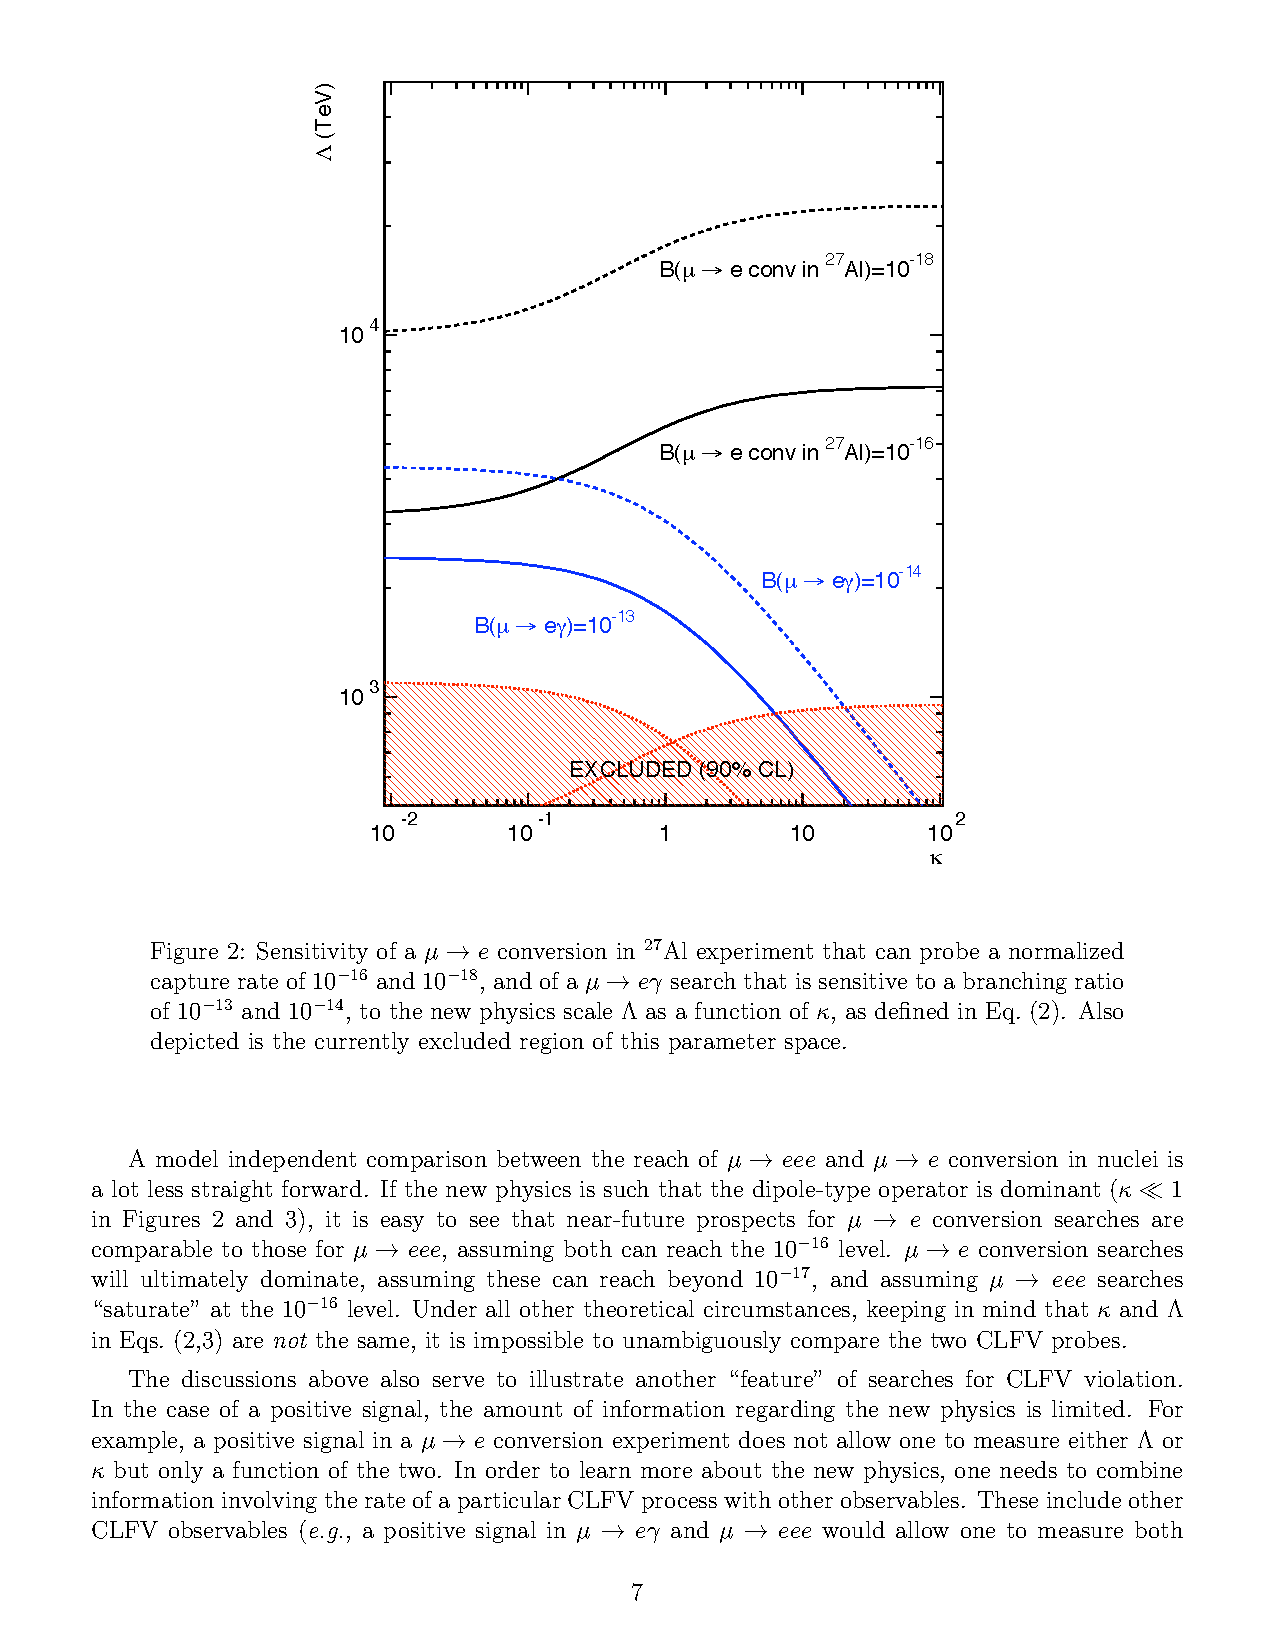
\includegraphics[trim = 45mm 130mm 50mm 10mm, clip, width=\linewidth]{Page7.pdf}
  \caption{{Sensitivity of a $\mu\to e$ conversion in $^{27}$Al experiment that can probe a normalized capture 
rate of $10^{−16}$ and $10^{−18}$, and of a $\mu \to e \gamma$ search that is sensitive to a branching ratio of $10^{−13}$ and 
$10^{−14}$, to the new physics scale $\Lambda$ as a function of $\kappa$, as defined in the text. Also depicted is the 
currently excluded region of this parameter space.
}}
\label{fig:cl:p7}
\end{minipage}
\hspace{0.3cm}
\begin{minipage}[b]{0.48\linewidth}
\centering
    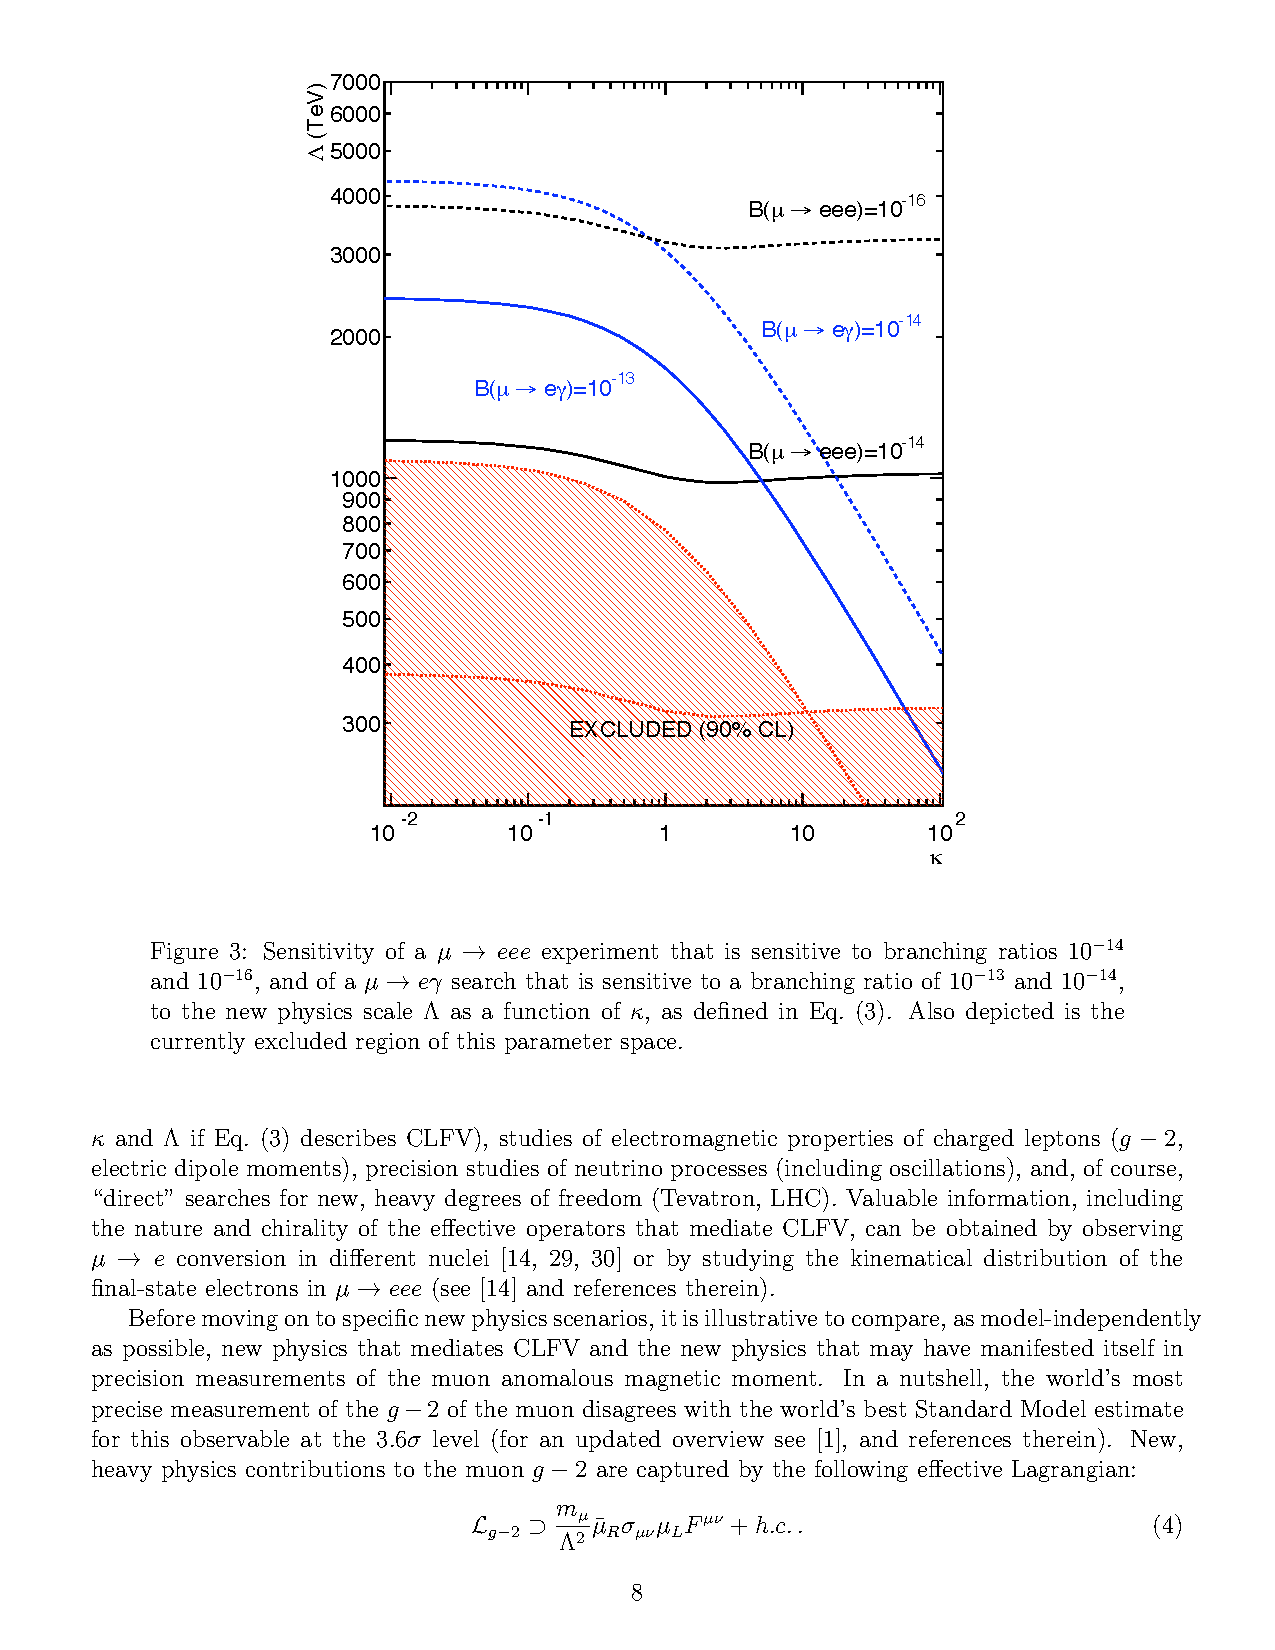
\includegraphics[trim = 45mm 130mm 50mm 10mm, clip, width=\linewidth]{Page8.pdf}
  \caption{{Sensitivity of a $\mu \to eee$ experiment that is sensitive to branching ratios $10^{−14}$ and 
$10^{−16}$, and of a $\mu \to e \gamma$ search that is sensitive to a branching ratio of $10^{−13}$ and $10^{−14}$, to the new 
physics scale $\Lambda$ as a function of $\kappa$, as defined in the text.  Also depicted is the
currently excluded region of this parameter space.
}}
  \label{fig:cl:p8}
\end{minipage}
\end{figure}

In general, muon measurements have the best
sensitivity over the largest range of the parameter space of many new
physics models. There are, however, models
in which  rare tau decays could provide the discovery
channel. It was clear from the discussion that as many different
CLFV searches as feasible should be conducted, since the best discovery
channel is model-dependent and the model is not yet known.  Should a
signal be observed in any channel, searches and measurements in as
many CLFV channels as possible will be crucial to determining the nature
of the underlying physics, since correlations between the rates
expected in different channels provide a powerful discriminator between
physics model.

The new muon $g\!\!-\!\!2$ experiment will measure the anomaly to close to 100 parts per billion precision
with different experimental techniques. This will be an important measurement whether or not the LHC sees new physics. If the LHC sees SUSY-like new physics, $g\!\!-\!\!2$ will be used as a constraint in determining which model we see. The LHC will be particularly sensitive to color super-partners, while $g\!\!-\!\!2$ can pin down the flavor sector. The sensitivity of $g\!\!-\!\!2$ to $\tan\beta$ will provide a test the universality of that parameter. If the LHC does not see new physics, then $g\!\!-\!\!2$ can be used to constrain other models, such as theories involving dark photons and extra dimensions. Any new physics model will have to explain the discrepancy between the theoretical and experimental values of $g\!\!-\!\!2$.
The reduction of theory errors in the calculation of $g\!\!-\!\!2$ is thus also of great importance, particularly the contribution of light-by-light scattering.  New data from the KLOE and BES-III experiments  will put the candidate models on firmer ground, as will lattice calculations to be undertaken by, among others, the USQCD collaboration. A Super $B$ Factory with a polarized electron beam can measure, for the first time, the anomalous moment of the $\tau$, using new variables involving the polarization.


The search for EDMs will also play an important role in new physics
searches. The achievable limit on the electron EDM is the most stringent, but searches for muon and tau EDMs are nonetheless of interest, since new physics contributions scale as the lepton mass. These can be
important: if an electron EDM were to be found, the value of second and third generation EDMs would be of great interest.  Parasitic measurements with the new Fermilab $g\!\!-\!\!2$ experiment will improve the $\mu$ EDM limit by two
orders of magnitude. Improvement of this limit would also help to rule out
the possibility that the muon EDM is the cause of the current discrepancy in the
$g\!\!-\!\!2$ measurement. New dedicated experiments now being discussed
could bring the limit down to the $10^{-24}$ $e$cm level, making it
competitive with the electron EDM constraints. In the same vein, a Super $B$ Factory with a polarized electron beam can reach a sensitivity below $10^{-21}$ $e$cm.
Additional symmetry tests will also be possible, including sensitive searches for $C\!P$ violation in $\tau$ decay and 
tests of electroweak parity violation using electron scattering and $e^+e^-$ collisions. 

An exciting program of sensitive searches for new physics using the large samples of $\mu$ and $\tau$ decays in experiments at the intensity frontier awaits us. These experiments will likely be central to our understanding of physics beyond the Standard Model.


\end{document}



